\documentclass[11pt,letterpaper,oneside]{scrartcl}

\usepackage{graphicx,mathtools,fixltx2e,amssymb}
\usepackage{tikz}

\title{Laplace transform with a Heaviside function}
\author{Nathan Grigg}
\date{}
\pagestyle{empty}
\usepackage[top=1in,bottom=1in]{geometry}

\setcounter{secnumdepth}{0}

\renewcommand{\L}[1]{\mathcal L\{#1\}}
\newcommand{\Lb}[1]{\mathcal L\Big\{#1\Big\}}
\newcommand{\Lbi}[1]{\mathcal L^{-1}\Big\{#1\Big\}}
\newcommand{\LL}[1]{\mathcal L\left\{#1\right\}}

\begin{document}
\begin{center}
	{\usekomafont{title}\LARGE Laplace transform with a Heaviside function}\\[10pt]
	by Nathan Grigg
\end{center}


\section{The formula}
To compute the Laplace transform of a Heaviside function
times any other function, use
\begin{equation*}
\boxed{\Lb{u_c(t) f(t)} = e^{-cs}\Lb{f(t+c)}.}
\end{equation*}
Think of it as a formula to get rid of the Heaviside function so that you
can just compute the Laplace transform of $f(t+c)$, which is doable.

In words: To compute the Laplace transform of
$u_c$ times $f$, shift $f$ left by $c$,
take the Laplace transform, and multiply the result by $e^{-cs}$.
Remember that to shift left, you replace $t$ with $t+c$.

\section{The other way to write the formula}

You will sometimes see the formula written as
$\L{u_c(t) f(t-c)} = e^{-cs}F(s),$
where $F(s)$ is the Laplace transform of $f(t)$.
This is a correct formula that says the same thing as the first
formula, but it is a \emph{terrible} way to compute the Laplace
transform. It is, however, a perfectly fine way to compute
the \emph{inverse} Laplace transform.
Rewrite it as
\begin{equation*}
	\boxed{\Lbi{e^{-cs} F(s)} = u_c(t)f(t-c).}
\end{equation*}

In words: To compute the inverse Laplace transform of $e^{-cs}$ times $F$,
find the inverse Laplace transform of $F$, call it $f$, then shift $f$ right
by $c$ and multiply by $u_c$.
Remember that to shift right, you replace $t$ with $t-c$.



\section{Why it works}

Right now you are probably thinking, \emph{Don't prove it to me! I trust you!}
Mathematicians believe that understanding a proof is crucial to understanding
a statement, because that's how our brains work. Sometimes we go a little too
far and forget that there are other great ways to understand math.

In this case, though, you should see the proof. It will help you understand. \emph{Trust me!}

\begin{align*}
	\Lb{u_c(t) f(t)} &= \int_0^\infty e^{-st} u_c(t) f(t) \, dt
 &&\text{definition of Laplace transform}\\
	&= \int_c^\infty e^{-st} f(t)\, dt &&\text{because the integral from $0$ to $c$ is $0$}\\
	&= \int_0^\infty e^{-s(t+c)} f(t+c)\,dt && \text{shift left by $c$}\\
	&= e^{-cs}\int_0^\infty e^{-st} f(t+c)\, dt &&\text{pull out constant $e^{-cs}$} \\
	&= e^{-cs}\Lb{f(t+c)} && \text{definition of Laplace transform}
\end{align*}

Here is the same thing in pictures:
\begin{center}
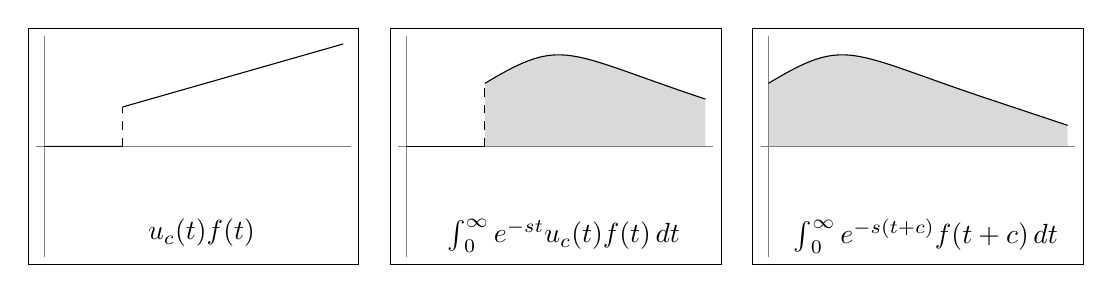
\begin{tikzpicture}
\draw (-0.2,-1.5) rectangle (4,1.5);
\draw[help lines] (0,-1.4) -- (0,1.4) (-0.1,0) -- (3.9,0);
\draw (0,0) -- (1,0) (1,0.5) -- (3.8,1.3);
\draw[dashed] (1,0) -- (1,0.5);
\draw (2,-0.8) node[below]{$u_c(t) f(t)$};

\begin{scope}[xshift=4.6cm]
\draw (-0.2,-1.5) rectangle (4,1.5);
\fill[gray!30] (1,0.8) .. controls (2,1.4) and (2,1.2) .. (3.8,0.6)
            -- (3.8,0) -- (1,0) -- cycle;
\draw[help lines] (0,-1.4) -- (0,1.4) (-0.1,0) -- (3.9,0);
\draw (0,0) -- (1,0);
\draw (1,0.8) .. controls (2,1.4) and (2,1.2) .. (3.8,0.6);
\draw[dashed] (1,0) -- (1,0.8);
\draw (2,-0.8) node[below]{$\int_{\,0}^\infty e^{-st} u_c(t)f(t)\,dt$};
\end{scope}

\begin{scope}[xshift=9.2cm]
\draw (-0.2,-1.5) rectangle (4,1.5);
\fill[gray!30] (0,0.8) .. controls (1,1.4) and (1,1.2) .. (2.8,0.6) --
(3.8,.2667)-- (3.8,0) -- (0,0) -- cycle;
\draw[help lines] (0,-1.4) -- (0,1.4) (-0.1,0) -- (3.9,0);
\draw (0,0.8) .. controls (1,1.4) and (1,1.2) .. (2.8,0.6) -- (3.8,.2667);
\draw (2,-0.8) node[below]{$\int^{\infty}_{\,0} e^{-s(t+c)} f(t+c)\,dt$};
\end{scope}
\end{tikzpicture}
\end{center}

The last integral simplifies to $e^{-cs}\L{f(t+c)}$ because at this
point we are treating $s$ as a constant.

Hopefully by looking at these pictures, you see the key idea:
\emph{Shifting left by $c$ allows us to get rid of the Heaviside function.}


\section{Some algebra required}

If $f(t)=t^2$, then $f(t+c)=(t+c)^2$. How do you take the Laplace
transform of $(t+c)^2$? You have to rearrange things,
in this case expanding to $t^2 + 2ct + c^2$.

Another example: If $f(t)=e^{2t}$ then
$f(t+c)=e^{2(t+c)}$. If you want to take the Laplace transform,
you need to expand to $e^{2t}e^{2c}$.

And a harder one: If $f(t)=\sin t$, then $f(t+c)=\sin(t+c)$.
If you want to take the Laplace transform, you need to do some
trigonometric magic. If $c$ is a multiple of $\pi/2$ or $\pi$,
you can probably figure it out by drawing some triangles.
Otherwise, pull out your trig identities!%
\footnote{You might need $\sin(t+c) = \cos(c)\sin(t) + \sin(c)\cos(t)$, or
maybe
$\cos(t+c) = \cos(c)\cos(t) - \sin(c)\sin(t)$.}

\section{This is not a product rule}

One common misconception about this Laplace transform
 formula is that it is a kind
of product rule, that the Laplace transform of $u_c(t)$ times $f(t)$ is the
Laplace transform of $u_c(t)$ times the Laplace transform of $f(t)$.
\emph{It is not! There is no product rule for Laplace transforms.}

Still not convinced? Here you go:
\begin{align*}
	\L{u_c(t)} &= \frac{e^{-cs}}{s}
	& \L{t} &= \frac{1}{s^2}
	& \L{u_c(t) \cdot t } &= e^{-cs}\left(\frac{1}{s^2} + \frac{c}{s}\right) \\
	\L{t} &= \frac{1}{s^2}
	& \L{t^2} &= \frac{2}{s^3}
	& \L{t\cdot t^2} &= \frac{6}{s^4}
\end{align*}

Once again, there is no product rule. There is only a fancy way to take
a step function from inside a Laplace transform operator and bring
it outside.

\end{document}
